Kiểm thử chấp nhận của người dùng (UAT) là một giai đoạn quan trọng trong quy trình phát triển phần mềm, trong đó phần mềm hoặc ứng dụng được người dùng cuối kiểm tra để đảm bảo rằng phần mềm hoặc ứng dụng đáp ứng nhu cầu của họ và sẵn sàng để phát hành sản xuất. Quy trình kiểm thử UAT giúp xác thực rằng hệ thống hoạt động chính xác, thân thiện với người dùng và đáp ứng các yêu cầu đã chỉ định.

Quá trình UAT bao gồm việc bao quát và xây dựng các kịch bản kiểm thử dựa trên yêu cầu người
dùng, sau đó người dùng cuối kiểm tra để đảm bảo sản phẩm hoạt động đúng như mong đợi và kịch
bản. UAT giúp giảm thiểu rủi ro, phát hiện lỗi quan trọng, tăng tính trải nghiệm và đảm bảo sự hài
lòng của người dùng khi sản phẩm được đưa vào sử dụng thực tế.

Để thực hiện UAT, nhóm thực hiện theo quy trình sau:
\begin{itemize}
    \item Phân tích yêu cầu và lập kế hoạch thử nghiệm:
    \begin{itemize}
        \item Xác định mục tiêu thực hiện UAT: kiểm thử sự chấp nhận người dùng đối với các tính năng và quá trình hoạt động của hệ thống, giao diện và trải nghiệm người dùng.
        \item Xác định đối tượng kiểm thử: người sử dụng đến từ các doanh nghiệp khác nhau và sinh viên.
        \item Lập kế hoạch thử nghiệm: thực hiện kiểm thử ngay một vài đối tượng bằng đường dẫn khảo sát Google Forms.
    \end{itemize}
    \item Thiết kế test case:
    \begin{itemize}
        \item Sử dụng các test case trong phần kiểm thử yêu cầu chức năng nhằm kiểm tra các chức năng có hoạt động đúng như mong đợi của người dùng không
    \end{itemize}
    \item Thiết lập môi trường và tiến hành thử nghiệm:
    \begin{itemize}
        \item Thực hiển triển khai hệ thống lên Internet để mọi đối tượng có thể sử dụng.
        \item Chuẩn bị một bài khảo sát kỹ lưỡng qua Google Forms nhằm thuận lợi trong việc lấy khảo sát người dùng từ xa
        \item Gửi bài khảo sác đến các đối tượng cần kiểm thử, đảm bảo sự trung thực và minh bạch để lấy được kết quả chính xác đến từ người dùng.
    \end{itemize}
    \item Báo cáo và nhận phản hồi
    \begin{itemize}
        \item Nếu phát hiện thấy bất kỳ sự cố hoặc lỗi nào, người dùng cuối gửi phản hồi ngay trên biểu mẫu khảo sát
        \item Nhóm phát triển sẽ xem xét và giải quyết các lỗi này, phát hành bản sửa lỗi khi cần.
    \end{itemize}
\end{itemize}

Và kết quả kiểm thử thu được như sau:
\begin{itemize}
    \item Tổng cộng 9 người dùng được kiểm thử với độ tuổi, nghề nghiệp và đến từ các công ty, doanh nghiệp khác nhau.
    \begin{figure}[H]
        \centering
        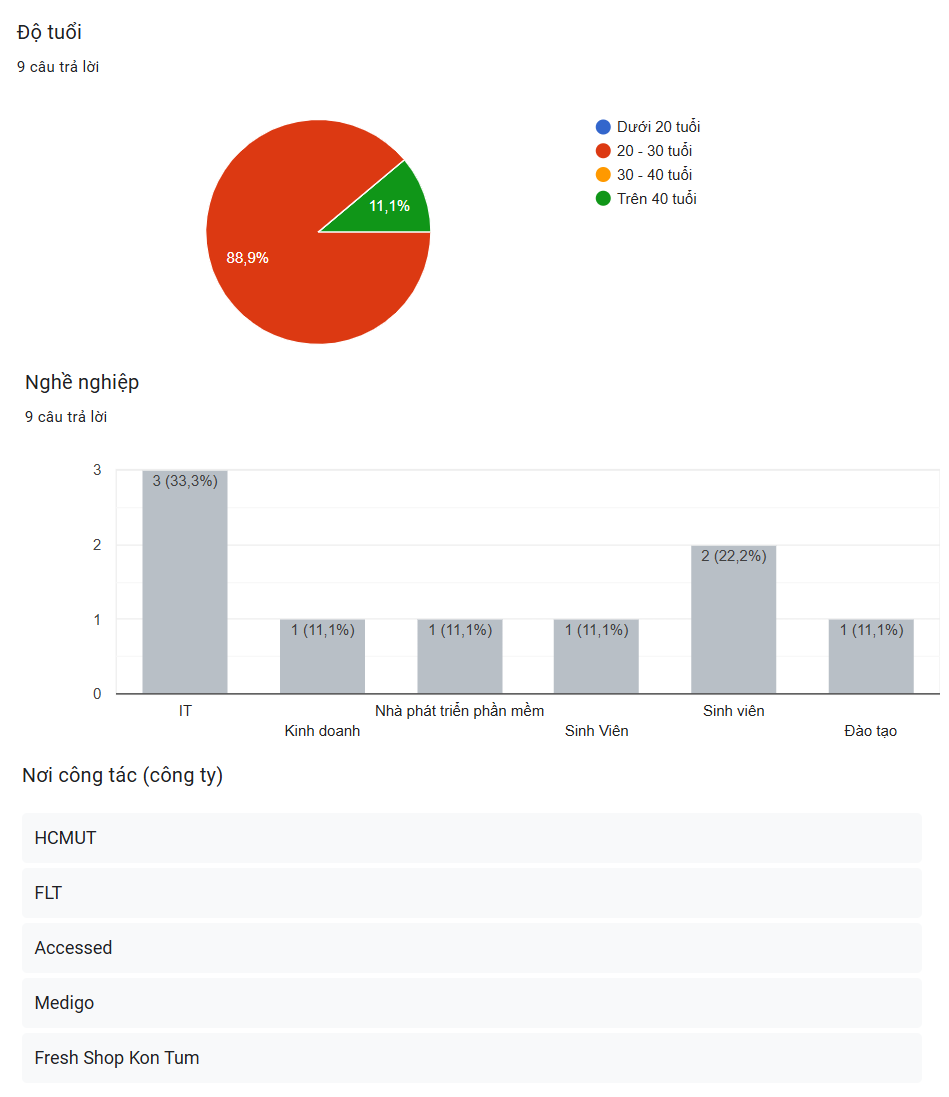
\includegraphics[width=0.8\textwidth]{Images/uat1.png}
        \vspace{0.5cm}
        \caption{Thống kê độ tuổi, nghề nghiệp và nơi công tác}
        \label{fig:enter-label}
    \end{figure}
    \item Nhóm đã cho người dùng đánh giá theo từng nhóm chức năng với thang điểm là 3
    \begin{figure}[H]
        \centering
        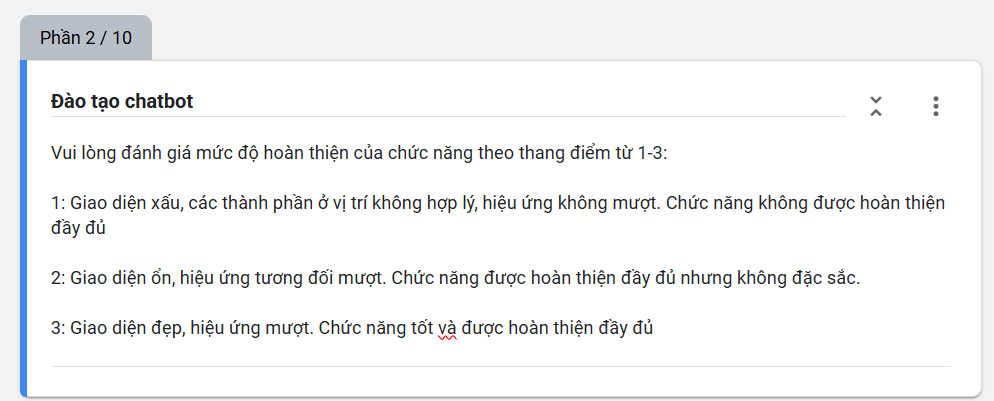
\includegraphics[width=0.8\textwidth]{Images/uat2.png}
        \vspace{0.5cm}
        \caption{Cách đánh giá chức năng}
        \label{fig:enter-label}
    \end{figure}

    Có tổng cộng là 52 testcase và 9 người dùng nên thu được 468 lượt cho điểm (trong đó 1 lượt 1 điểm, 97 lượt 2 điểm và 370 lượt 3 điểm)
    \begin{figure}[H]
        \centering
        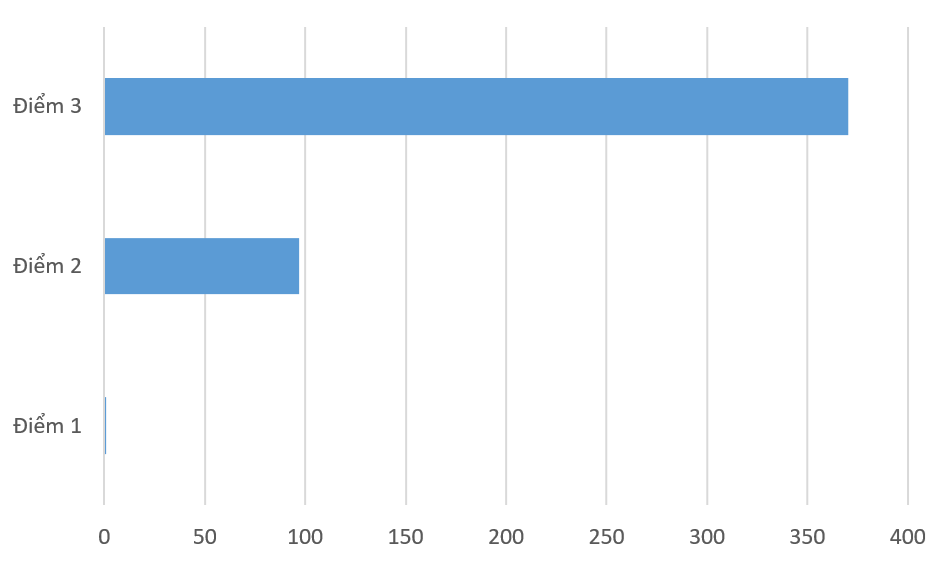
\includegraphics[width=0.8\textwidth]{Images/uat3.png}
        \vspace{0.5cm}
        \caption{Thống kê đánh giá theo thang điểm của người dùng}
        \label{fig:enter-label}
    \end{figure}
    \item Ngoài ra, hệ thống còn nhận thêm những lời nhận xét và góp ý nhằm cải thiện hệ thống hơn
    \begin{figure}[H]
        \centering
        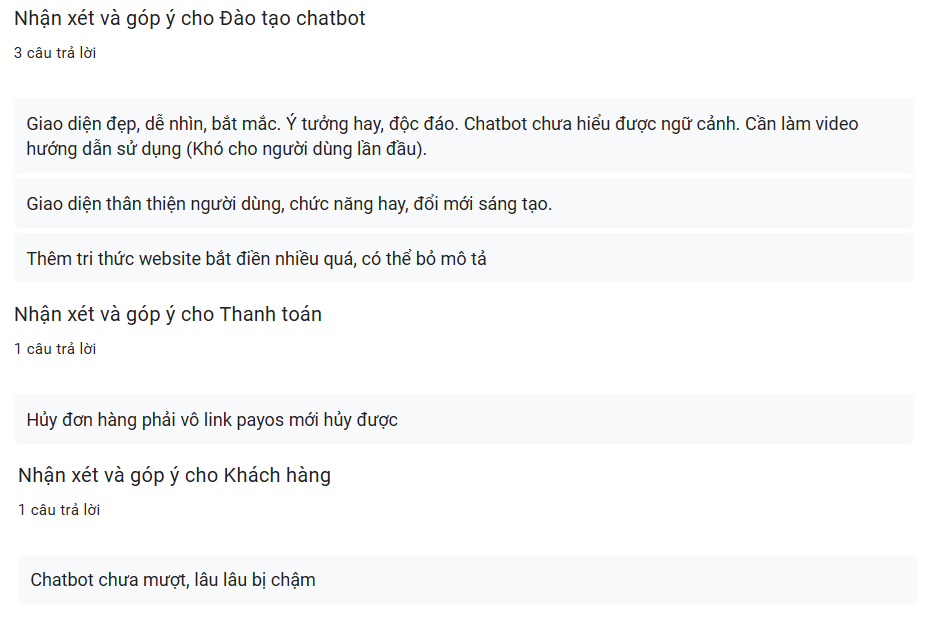
\includegraphics[width=1\textwidth]{Images/uat4.png}
        \vspace{0.5cm}
        \caption{Những nhận xét, góp ý từ người dùng}
        \label{fig:enter-label}
    \end{figure}
    \item Bên dưới là thống kê các đánh giá tổng quan về hệ thống
    \begin{figure}[H]
        \centering
        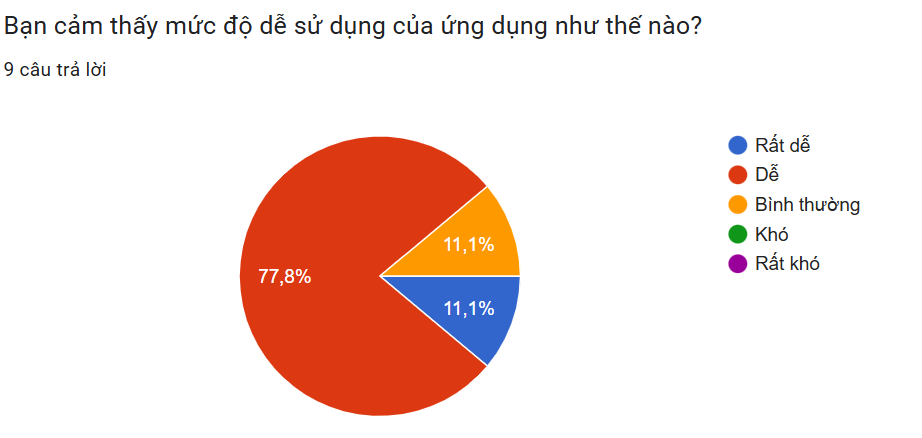
\includegraphics[width=0.8\textwidth]{Images/uat5.png}
        \vspace{0.5cm}
        \caption{Thống kê đánh giá mức độ dễ sử dụng}
        \label{fig:enter-label}
    \end{figure}
    \begin{figure}[H]
        \centering
        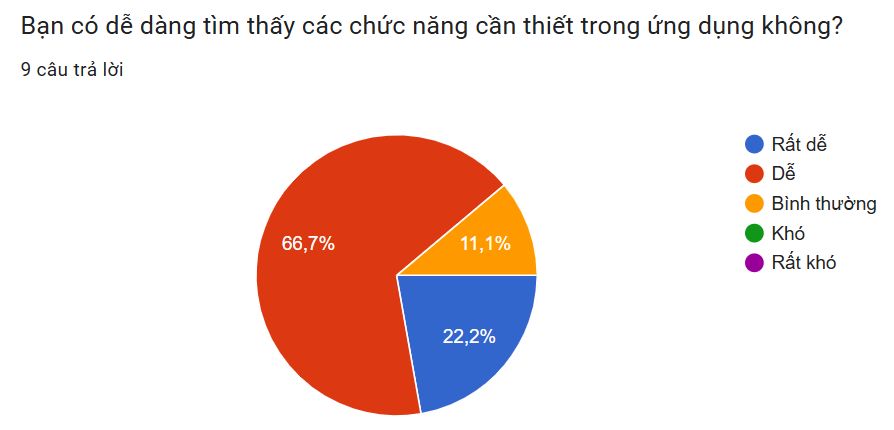
\includegraphics[width=0.8\textwidth]{Images/uat6.png}
        \vspace{0.5cm}
        \caption{Thống kê đánh giá mức độ dễ tìm thấy chức năng}
        \label{fig:enter-label}
    \end{figure}
    \begin{figure}[H]
        \centering
        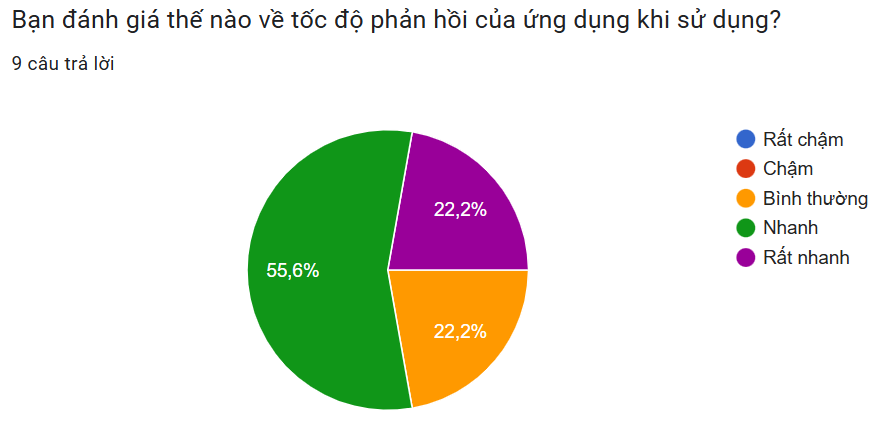
\includegraphics[width=0.8\textwidth]{Images/uat7.png}
        \vspace{0.5cm}
        \caption{Thống kê đánh giá tốc độ phản hồi}
        \label{fig:enter-label}
    \end{figure}
    \begin{figure}[H]
        \centering
        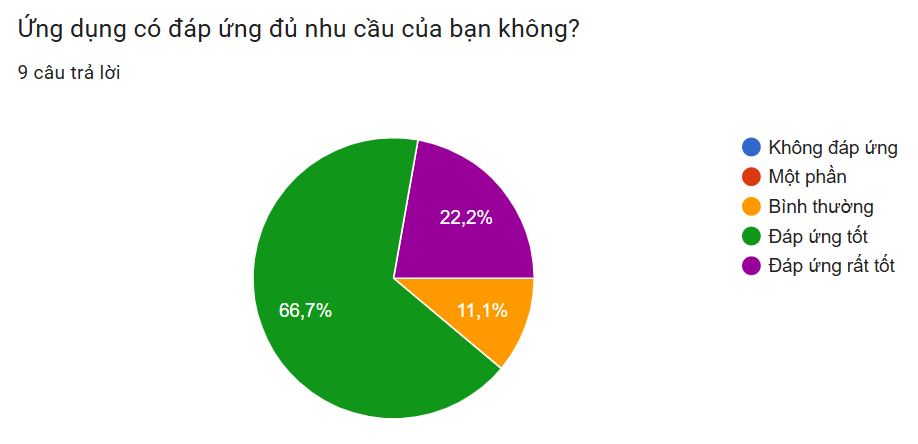
\includegraphics[width=0.8\textwidth]{Images/uat8.png}
        \vspace{0.5cm}
        \caption{Thống kê đánh giá khả năng đáp ứng}
        \label{fig:enter-label}
    \end{figure}
    \begin{figure}[H]
        \centering
        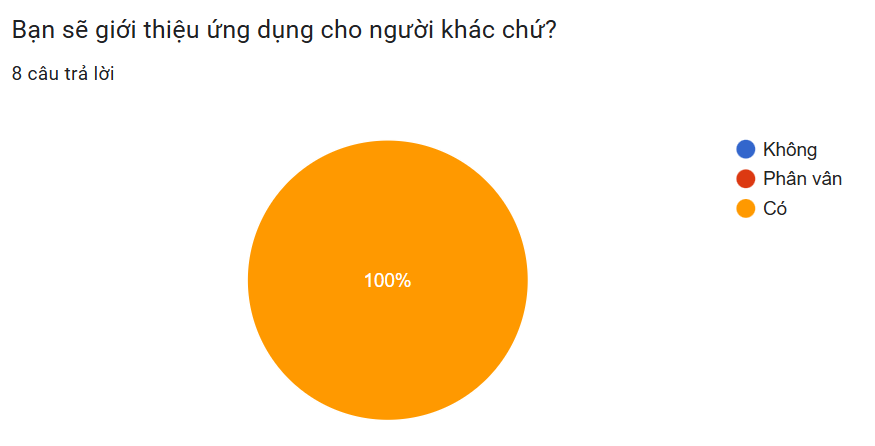
\includegraphics[width=0.8\textwidth]{Images/uat9.png}
        \vspace{0.5cm}
        \caption{Thống kê đánh giá khả năng giới thiệu}
        \label{fig:enter-label}
    \end{figure}
\end{itemize}
